% 来源：固定1991上海PDF第3页（印刷5-35），第26题。
% 根据已给条件数学化重建，绘图例取L:y=-3(x-2)/2，非新增题设。
% B=(1/2,9/4), C=(-2,6), P=(-2/11,36/11), Q=(20/33,12/11)。
% 精确检查：BP/PC=(9/4)/6=3/8，Q为POA重心。
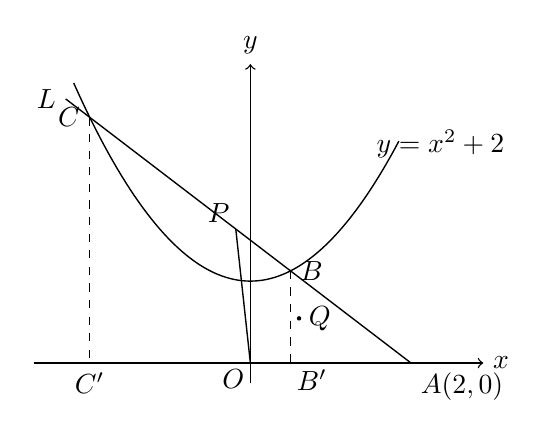
\begin{tikzpicture}[x=1.02cm,y=0.52cm,line width=0.5pt]
  \coordinate (O) at (0,0);
  \coordinate (A) at (2,0);
  \coordinate (B) at ({1/2},{9/4});
  \coordinate (C) at (-2,6);
  \coordinate (Bp) at ({1/2},0);
  \coordinate (Cp) at (-2,0);
  \coordinate (P) at ({-2/11},{36/11});
  \coordinate (Q) at ({20/33},{12/11});
  \draw[->] (-2.7,0)--(2.9,0) node[right] {$x$};
  \draw[->] (0,-0.5)--(0,7.3) node[above] {$y$};
  \draw[domain=-2.2:1.85,samples=80,smooth] plot (\x,{\x*\x+2});
  \draw (-2.3,6.45)--(A);
  \draw (P)--(O);
  \draw[dashed] (B)--(Bp);
  \draw[dashed] (C)--(Cp);
  \fill (Q) circle[radius=0.8pt];
  \node[below left,inner sep=2pt] at (O) {$O$};
  \node[below right] at (A) {$A(2,0)$};
  \node[right] at (B) {$B$};
  \node[left] at (C) {$C$};
  \node[below right,inner sep=2pt] at (Bp) {$B'$};
  \node[below] at (Cp) {$C'$};
  \node[above left,inner sep=2pt] at (P) {$P$};
  \node[right] at (Q) {$Q$};
  \node[left] at (-2.3,6.45) {$L$};
  \node[right] at (1.45,5.35) {$y=x^2+2$};
\end{tikzpicture}
